\documentclass{article}


\usepackage[margin=1in]{geometry}
\usepackage{amsmath}
\usepackage{graphicx}
\usepackage{tabu}
\usepackage{listings}
\usepackage{color}

\author{Zachary Vogel}
\title{Numerical Analysis Homework 4\\ APPM 4650}
\date{\today}

\begin{document}

\definecolor{keywords}{RGB}{255,0,90}
\definecolor{comments}{RGB}{0,0,113}
\definecolor{red}{RGB}{160,0,0}
\definecolor{green}{RGB}{0,150,0}
 
\lstset{language=Python, basicstyle=\ttfamily\small, keywordstyle=\color{keywords}, commentstyle=\color{comments},stringstyle=\color{red},showstringspaces=false,identifierstyle=\color{green}}



\maketitle


\section*{Problem 1}
The first problem asks for an approximation to the integral $\int_0^1x^2e^{-x}dx$ using Guassian Quadrature using $n=3$. It also asks for a comparison of the results to the exact value of the integral.\\
First, rewriting the integral we get:
\[\alpha=\int_0^1x^2e^{-x}dx=\frac{1}{2}\int_{-1}^1\left (\frac{1}{2}x+\frac{1}{2}\right )^2e^{-\left (\cfrac{1}{2}x+\cfrac{1}{2}\right )}dx\]
Then, we use our weights and evaluations to estimate with 3 points:
\[\alpha=\frac{1}{2}\left (\frac{8}{9}\frac{1}{4}e^{-\cfrac{1}{2}}+\frac{5}{9}\left (\left (\frac{1}{2}\sqrt{\frac{3}{5}}+\frac{1}{2}\right )^2e^{-\left(\cfrac{1}{2}\sqrt{\cfrac{3}{5}}+\cfrac{1}{2}\right)}+\left (-\frac{1}{2}\sqrt{\frac{3}{5}}+\frac{1}{2}\right )^2e^{\cfrac{1}{2}\sqrt{\cfrac{3}{5}}-\cfrac{1}{2}}\right )\right )\]
Solving, we get that the integral is approximately $\alpha=0.160595$. The actual value wolfram alpha gave me was $0.16060$. Therefore, we are really really close to the exact value from a 3 point approximation.

\section*{Problem 2}
Here, use Runge-Kutta 4 to approximate the solution to the following first order system of equations for $0\leq t\leq 1$, and $h=0.2$. It also wants a comparison to the actual solution. The system is defined by:
\[u'_1=3u_1+2u_2-(2t^2+1)e^{2t}\quad u_1(0)=1\]
\[u'_2=4u_1+u_2+(t^2+2t-4)e^{2t}\quad u_2(0)=1\]
The exact solutions for this problem are:
\[u_1(t)=\frac{1}{3}e^{5t}-\frac{1}{3}e^{-t}+e^{2t}\]
\[u_2(t)=\frac{1}{3}e^{5t}+\frac{2}{3}e^{-t}+t^2e^{2t}\]
I solved this problem with a python script that I wrote. The code for it is in Appendix 1, here is the table of results for the problem.
\begin{figure}[h!]
    \centering
    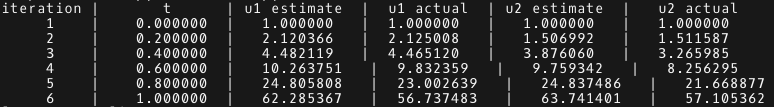
\includegraphics[width=0.9\textwidth]{Prob2.png}
\end{figure}
The problem of methods like this is visible. As the iteration number increases, the error gets bigger with every step.

\section*{Problem 3}
Here, we are again given a differential equation, $y'=x+y$ with $y(0)=0$. Find $y(x)$ for $0\leq x\leq 0.5$ with a step size of $h=0.1$. It wants the solution using several different methods, while noting that any seed values can be approximated by $y\approx \frac{x^2}{2}$ when $x<<1$.
\subsection*{(a)}
First, the solution with Runge-Kutta 4.\\
Once again, I used a python script I wrote to solve this problem. The code is in Appendix 2, here are the results.\\
\begin{figure}[h!]
    \centering
    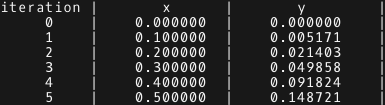
\includegraphics[width=0.7\textwidth]{Prob31.png}
\end{figure}
\subsection*{(b)}
Next with the improved Euler method.\\
Yay, python scripts. Here are the results, code is in Appendix 3:
\begin{figure}[h!]
    \centering
    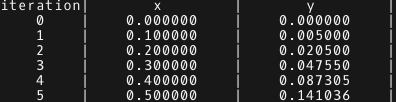
\includegraphics[width=0.7\textwidth]{Prob32.png}
\end{figure}
\subsection*{(c)}
Finally, solve with the Predictor-corrector using the Adams-bashforth 4-step for the predictor and the Adams-Moulton 3-step as the corrector. Again I implemented in python. I didn't want to do boring things with the seed values, so my code is relatively unusual (various step sizes until I have enough seed values). Here is the table of results, the code is in Appendix 4. This doesn't seem correct, probably because of my attempt at a good way to iterate.
\begin{figure}[h!]
    \centering
    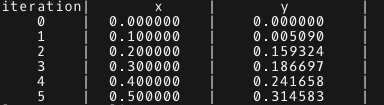
\includegraphics[width=0.7\textwidth]{Prob33.png}
\end{figure}
\clearpage
\appendix
\section{Appendix 1}
\lstinputlisting{rk4_P2.py}
\section{Appendix 2}
\lstinputlisting{rk4_P3.py}
\section{Appendix 3}
\lstinputlisting{impeul_P3.py}
\section{Appendix 4}
\lstinputlisting{PRCR.py}

\end{document}
